%!TEX root = ../main.tex



\section{Εισαγωγή στους PID ελεγκτές}

\lettrine[findent=2pt]{\fbox{\textbf{Έ}}}{νας} αναλογικός-ολοκληρωτικός-παραγωγικός ελεγκτής (\emph{proportional-integral-derivative controller}) ή όπως είναι πιο γνωστός \emph{PID controller}, είναι ένας μηχανισμός ανάδρασης (\emph{feedback}) βρόχου ελέγχου (\emph{control loop}) που χρησιμοποιείται ευρέως σε βιομηχανικά συστήματα ελέγχου καθώς και σε μια ποικιλία άλλων εφαρμογών που απαιτούν συνεχή διαμορφωμένο έλεγχο. Η διαδικασία λειτουργίας είναι κοινή για όλους τους ελεγκτές αυτού του είδους. Ένας PID ελεγκτής υπολογίζει συνεχώς μια τιμή σφάλματος $e(t)$ ως διαφορά μεταξύ μιας επιθυμητής τιμής ρύθμισης (\emph{setpoint} ή \emph{SP}) και μεταξύ μιας μεταβλητής της διαδικασίας ύπο έλεγχο (\emph{process value} ή \emph{PV}) και εφαρμόζει μια διόρθωση βασισμένη στον αναλογικό, ολοκληρωτικό και παραγωγικό όρο του (\emph{P}, \emph{I}, \emph{D} αντίστοιχα) οι οποίοι δίνουν και στον ελεγκτή το όνομά του.\\
\linebreak
Στην πράξη, εφαρμόζει αυτόματα διορθωμένη και ακριβή διόρθωση σε μια λειτουργία ελέγχου. Ένα καθημερινό παράδειγμα είναι ο έλεγχος ταχύτητας σε οδικό όχημα. όπου εξωτερικές επιδράσεις, όπως κλίσεις, θα προκαλούσαν αλλαγές στην ταχύτητα του οχήματος. Ο αλγόριθμος PID επαναφέρει την ταχύτητα του αυτοκινήτου στην επιθυμητή από τον οδηγό τιμή της με τον βέλτιστο τρόπο, χωρίς καθυστέρηση ή υπέρβαση, ελέγχοντας την ισχύ εξόδου του κινητήρα του οχήματος.

\subsection{Ιστορική αναδρομή}

\subsubsection{Προέλευση}
Ο συνεχής έλεγχος, προτού καταστούν πλήρως κατανοητοί και εφαρμοσμένοι οι ελεγκτές PID, έχει μία από τις πηγές του στον φυγοκεντρικό ρυθμιστή ο οποίος χρησιμοποιεί περιστρεφόμενα βάρη για να ελέγξει μια διαδικασία. Αυτό είχε εφευρεθεί από τον Christian Huygens τον 17ο αιώνα για να ρυθμίσει το χάσμα μεταξύ των μυλόπετρων στους ανεμόμυλους ανάλογα με την ταχύτητα περιστροφής και έτσι να αντισταθμίσει την μεταβλητή ταχύτητα της τροφοδότησης των σιτηρών \cite{origin1}, \cite{origin2}.

Με την εφεύρεση της σταθερής ατμομηχανής υψηλής πίεσης, υπήρχε ανάγκη για αυτόματο έλεγχο ταχύτητας και ο αυτοδιαμορφωμένος ρυθμιστής ``κωνικού εκκρεμούς" του James Watt, ένα σύνολο περιστρεφόμενων χαλύβδινων σφαιρών προσαρτημένων σε κάθετο άξονα με βραχίονες σύνδεσης, έγινε πρότυπο της βιομηχανίας \cite{origin3}.

Ωστόσο, ο περιστρεφόμενος έλεγχος ταχύτητας του ρυθμιστή εξακολουθούσε να είναι μεταβλητός υπό συνθήκες μεταβαλλόμενου φορτίου, και έτσι το μειονέκτημα του ελέγχου που πλέον είναι γνωστός ως αναλογικός έγινε προφανές. Το σφάλμα μεταξύ της επιθυμητής ταχύτητας και της πραγματικής ταχύτητας αυξανόταν με την αύξηση του φορτίου. Τον $19^o$ αιώνα, η θεωρητική βάση για τη λειτουργία των ρυθμιστών περιγράφηκε για πρώτη φορά από τον James Clerk Maxwell το $1868$. Εξερεύνησε τη μαθηματική βάση για τη σταθερότητα του ελέγχου και προχώρησε σε έναν καλό δρόμο προς μια λύση, αλλά έκανε μια έκκληση σε μαθηματικούς να εξετάσουν το πρόβλημα \cite{origin3}, \cite{origin4}. Το πρόβλημα εξετάστηκε περαιτέρω από τον Edward Routh το $1874$, τον Charles Sturm και το $1895$ από τον Adolf Hurwitz, που όλοι συνέβαλαν στην καθιέρωση κριτηρίων σταθερότητας ελέγχου \cite{origin3}. Στην πράξη, οι ρυθμιστές ταχύτητας βελτιώθηκαν περαιτέρω, κυρίως από τον αμερικανικό επιστήμονα Willard Gibbs, ο οποίος το $1872$ ανέλυσε θεωρητικά τον κωνικό κυβερνήτη εκκρεμούς του Watt.

Περίπου εκείνη την εποχή, η εφεύρεση της τορπίλης Whitehead έθεσε ένα πρόβλημα ελέγχου το οποίο απαιτούσε ακριβή έλεγχο του βάθους λειτουργίας. Η χρήση μόνο ενός αισθητήρα πίεσης βάθους αποδείχθηκε ανεπαρκής και έτσι ένα εκκρεμές που μετρούσε το εμπρόσθιο και οπίσθιο βήμα της τορπίλης συνδυάστηκε με τη μέτρηση βάθους για να γίνει ο έλεγχος εκκρεμούς και υδροστάτη (\emph{pendulum-and-hydrostat control}). Ο έλεγχος πίεσης παρείχε μόνο ένα αναλογικό έλεγχο, το οποίο αν το κέρδος ελέγχου ήταν πολύ υψηλό, θα ήταν ασταθές και θα έπεφτε σε υπέρβαση, με σημαντική αστάθεια στη διατήρηση βάθους. Το εκκρεμές προσέθεσε αυτό που είναι τώρα γνωστό ως παράγωγο έλεγχο (\emph{derivative control}), το οποίο εξασθένισε τις ταλαντώσεις ανιχνεύοντας τη γωνία κατάδυσης / ανόδου της τορπίλης και επομένως τον ρυθμό μεταβολής του βάθους \cite{origin5}. Αυτή η εξέλιξη (που ονομάστηκε από το Whitehead ως ``\emph{Το Μυστικό}" για να μην δώσει καμιά ένδειξη για τη δράση της) ήταν περίπου το $1868$ \cite{origin6}.

Ένα άλλο πρώιμο παράδειγμα ελεγκτή τύπου PID αναπτύχθηκε από τον Elmer Sperry το $1911$ για την πλοήγηση, αν και το έργο του ήταν διαισθητικό και όχι μαθηματικό \cite{origin7}.

Η πρώτη θεωρητική ανάλυση και πρακτική εφαρμογή αφορούσε το αυτόματο σύστημα διεύθυνσης πλοίων, το οποίο αναπτύχθηκε από τις αρχές της δεκαετίας του $1920$ και μετά από τον μηχανικό Nicolas Minorsky \cite{origin8}. Ο Minorsky ερευνούσε και σχεδίαζε την αυτόματη καθοδήγηση πλοίων για το Πολεμικό Ναυτικό των ΗΠΑ και βάσισε την ανάλυσή του στις παρατηρήσεις ενός πηδαλιούχου. Σημείωσε ότι ο πηδαλιούχος κατεύθυνε το πλοίο με βάση όχι μόνο το τρέχον σφάλμα πορείας, αλλά και το λάθος του παρελθόντος, καθώς και τον τρέχοντα ρυθμό αλλαγής \cite{origin9}. Αυτό μοντελοποιήθηκε μαθηματικά από τον Minorsky \cite{origin3}. Ο στόχος του ήταν η σταθερότητα, όχι ο γενικός έλεγχος, ο οποίος απλοποίησε σημαντικά το πρόβλημα. Ενώ ο αναλογικός έλεγχος παρείχε σταθερότητα έναντι μικρών διαταραχών, ήταν ανεπαρκής για να αντιμετωπίσει μια σταθερή διαταραχή (λόγω σφάλματος σταθερής κατάστασης), η οποία απαιτούσε την προσθήκη του ολοκληρωτικού όρου. Τέλος, ο παράγωγος όρος προστέθηκε για να βελτιώσει τη σταθερότητα και τον έλεγχο.

Διεξήχθησαν δοκιμές στο USS New Mexico, με τον ελεγκτή να ελέγχει τη γωνιακή ταχύτητα (όχι τη γωνία) του πηδαλίου. Ο έλεγχος PI απέδωσε σταθερή στροφή (γωνιακό σφάλμα) $±2\degree$. Η προσθήκη του στοιχείου D οδήγησε σε σφάλμα εκτροπής $±{1/6}\degree$, καλύτερα από ότι θα μπορούσαν να επιτύχουν οι περισσότεροι πηδαλιούχοι \cite{origin10}.

Το Πολεμικό Ναυτικό τελικά δεν υιοθέτησε το σύστημα, λόγω της αντίστασης του προσωπικού. Παρόμοια εργασία πραγματοποιήθηκε και δημοσιεύθηκε από αρκετούς άλλους στη δεκαετία του $1930$.

\subsubsection{Βιομηχανικός έλεγχος}
Η ευρεία χρήση των ελεγκτών ανάδρασης δεν κατέστη εφικτή μέχρις ότου αναπτύχθηκαν ενισχυτές υψηλού κέρδους και μεγάλης ζώνης (\emph{wideband high-gain amplifiers}) για να χρησιμοποιηθεί η έννοια της αρνητικής ανάδρασης. Αυτοί είχαν αναπτυχθεί στην ηλεκτρονική τηλεφωνική μηχανική από τον Harold Black στα τέλη της δεκαετίας του $1920$, αλλά δεν δημοσιεύθηκε μέχρι το $1934$ \cite{origin3}. Ανεξάρτητα, ο Clesson E Mason της εταιρείας Foxboro, το $1930$, εφηύρε έναν ευρείας ζώνης πνευματικό ελεγκτή, συνδυάζοντας τον πνευματικό ενισχυτή με ακροφύσιο και πτερύγιο υψηλού κέρδους, που είχε εφευρεθεί το $1914$, με αρνητική ανάδραση από την έξοδο του ελεγκτή. Αυτό αύξησε δραματικά το γραμμικό εύρος λειτουργίας του ακροφυσίου και του ενισχυτή πτερυγίου και ο ολοκληρωμένος έλεγχος μπορούσε επίσης να προστεθεί με τη χρήση μιας βαλβίδας εξαέρωσης ακριβείας και ενός φυσητήρα. Το αποτέλεσμα ήταν ο ελεγκτής "Stabilog" ο οποίος έδωσε αναλογικές και ολοκληρωμένες λειτουργίες χρησιμοποιώντας ανατροφοδοτούμενους φυσητήρες \cite{origin3}. Αργότερα ο παράγωγος όρος προστέθηκε από ένα άλλο φυσητήρα και ρυθμιζόμενο στόμιο.

Από το $1932$ και μετά, η χρήση ευρυζωνικών ελεγκτών αυξήθηκε ραγδαία σε ποικίλες εφαρμογές ελέγχου. Ο πεπιεσμένος αέρας χρησιμοποιήθηκε τόσο για την παραγωγή της εξόδου του ελεγκτή όσο και για την τροφοδοσία της συσκευής διαμόρφωσης της διαδικασίας, όπως μια βαλβίδα ελέγχου που λειτουργεί με διαφράγματα. Ήταν απλές συσκευές χαμηλής συντήρησης που λειτουργούσαν καλά σε σκληρό βιομηχανικό περιβάλλον και δεν παρουσίαζαν κίνδυνο έκρηξης σε επικίνδυνες τοποθεσίες. Ήταν το βιομηχανικό πρότυπο για πολλές δεκαετίες μέχρι την εμφάνιση διακριτών ηλεκτρονικών ελεγκτών και κατανεμημένων συστημάτων ελέγχου.

\begin{figure}[h]
  \centering
  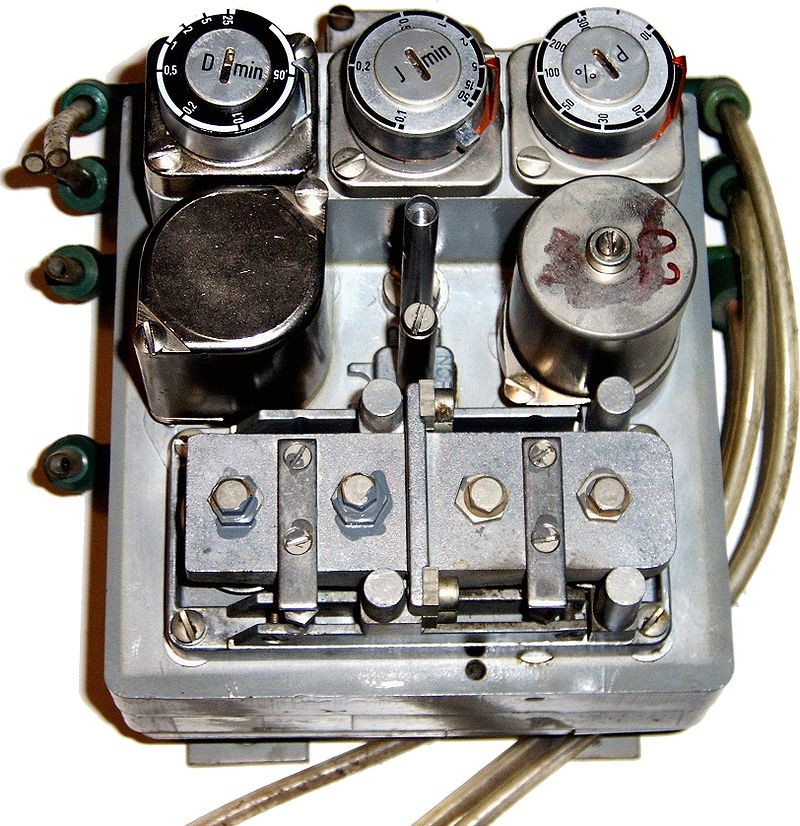
\includegraphics[width=\textwidth]{pneumatic_pid}
  \caption{Πνευματικός ελεγκτής PID. Οι συντελεστές των "τριών όρων" Ρ, Ι και D ρυθμίζονται από τους διακόπτες στην κορυφή}
  \label{fig:pneumatic_pid}
\end{figure}

Στη δεκαετία του $1950$, όταν οι ηλεκτρονικοί ενισχυτές υψηλού κέρδους έγιναν φτηνοί και αξιόπιστοι, οι ηλεκτρονικοί ελεγκτές PID έγιναν δημοφιλείς και χρησιμοποιήθηκαν σήματα ρεύματος βρόχου $4-20 mA$ τα οποία εξομοιώνουν το πνευματικό πρότυπο. Ωστόσο, οι ενεργοποιητές πεδίου (\emph{field actuators}) εξακολουθούν να χρησιμοποιούν ευρέως το πνευματικό πρότυπο λόγω των πλεονεκτημάτων της πνευματικής κινητήριας δύναμης για τις βαλβίδες ελέγχου στα περιβάλλοντα των μονάδων επεξεργασίας.

\subsubsection{Ηλεκτρονικοί αναλογικοί ελεγκτές}
Οι ηλεκτρονικοί αναλογικοί βρόχοι ελέγχου PID βρίσκονταν συχνά μέσα σε πιο σύνθετα ηλεκτρονικά συστήματα, όπως για παράδειγμα η τοποθέτηση της κεφαλής μιας μονάδας σκληρού δίσκου, η ρύθμιση της ισχύος ενός τροφοδοτικού ή ακόμα και το κύκλωμα ανίχνευσης κίνησης ενός σύγχρονου σεισμομέτρου. Οι διακριτοί ηλεκτρονικοί αναλογικοί ελεγκτές έχουν αντικατασταθεί σε μεγάλο βαθμό από ψηφιακούς ελεγκτές που χρησιμοποιούν μικροελεγκτές ή FPGA, για την εφαρμογή αλγορίθμων PID. Ωστόσο, διακριτοί αναλογικοί ελεγκτές PID εξακολουθούν να χρησιμοποιούνται σε εξειδικευμένες εφαρμογές που απαιτούν απόδοση υψηλού εύρους ζώνης και χαμηλού θορύβου, όπως ελεγκτές με λέιζερ-δίοδο \cite{origin11}.

%Στη συνέχεια χρησιμοποιήθηκε για τον αυτόματο έλεγχο της διαδικασίας στη μεταποιητική βιομηχανία, όπου εφαρμόστηκε ευρέως σε πνευματικούς, και στη συνέχεια ηλεκτρονικούς, ελεγκτές. Σήμερα υπάρχει γενική χρήση της ιδέας PID σε εφαρμογές που απαιτούν ακριβή και βελτιστοποιημένο αυτόματο έλεγχο.

\subsection{Χρησιμότητα PID ελεγκτών}

Ο PID ελεγκτής έχει διάφορα σημαντικά χαρακτηριστικά: παρέχει ανατροφοδότηση ελέγχου, έχει την ικανότητα να εξαλείφει το σφάλμα μόνιμης κατάστασης (\emph{steady-state error}) μέσω του ολοκληρωτικού του όρου, μπορεί να προβλέπει το μελλοντικό σφάλμα μέσω του παραγωγικού του όρου. Οι PID ελεγκτές παρέχουν ικανοποιητικό έλεγχο σε πολλά προβλήματα ελέγχου, ειδικά όταν οι δυναμικές που διέπουν τη διεργασία είναι ήπιες και οι απαιτήσεις ελέγχου μέτριες. Οι ελεγκτές αυτού του είδους έρχονται σε αρκετές διαφορετικές μορφές. Υπάρχουν αυτόνομα συστήματα μέσα σε κουτιά για έναν ή περισσότερους βρόχους και παράγονται εκατοντάδες χιλιάδες μονάδες κάθε χρόνο. Ο PID έλεγχος είναι σημαντικό στοιχείο ενός κατανεμημένου συστήματος ελέγχου. Οι ελεγκτές είναι επίσης ενσωματωμένοι σε πολλά, ειδικού σκοπού, συστήματα ελέγχου. Στον έλεγχο διεργασιών (\emph{process control}), περισσότερο από το $95\%$ των βρόχων ελέγχου είναι PID τύπου (οι περισσότεροι βρόχοι είναι στην πραγματικότητα PI ελέγχου).

Η δημοτικότητα του PID οφείλεται σε μεγάλο βαθμό στην ευκολία εφαρμογής και την αποτελεσματικότητά του. Το κίνητρο για τη χρήση του PID προέρχεται από την αποδοτικότητα του κόστους υλοποίησής του: ο ελεγκτής PID σπάνια αποτελεί ένα βέλτιστο ελεγκτή αλλά είναι αρκετά καλός στις περισσότερες περιπτώσεις και έτσι το πρόσθετο κόστος και η πολυπλοκότητα ενός βέλτιστου ελεγκτή δεν αξίζουν την οριακή αύξηση στην απόδοση. Επιπλέον, ο έλεγχος PID δεν απαιτεί βαθιά κατανόηση των υποκείμενων λειτουργιών μιας διαδικασίας. Το μόνο που έχει σημασία είναι ότι μερικές μετρούμενες μεταβλητές της διαδικασίας να μπορούν να επηρεαστούν έντονα από ορισμένες ελεγχόμενες μεταβλητές. Επίσης ένας PID ελεγκτής μπορεί εύκολα να μεταφερθεί από διεργασία σε διεργασία. Το μόνο που χρειάζεται είναι να προσαρμοστούν τα κέρδη των όρων του και τα όρια της εξόδου του έτσι ώστε να ταιριάζουν στην καινούρια διεργασία. Ο PID έλεγχος χρησιμοποιείται στο χαμηλότερο επίπεδο: ο πολλαπλών μεταβλητών ελεγκτής (\emph{multivariable controller}) δίνει το σημείο λειτουργίας στους ελεγκτές στο χαμηλότερο επίπεδο. Ο PID ελεγκτής μπορεί λοιπόν να ειπωθεί ότι αποτελεί το ``ψωμί και βούτυρο" της μηχανικής ελέγχου. Είναι, συνεπώς, ένα σημαντικό στοιχείο στην εργαλειοθήκη κάθε μηχανικού ελέγχου. 

Οι PID ελεγκτές έχουν επιβιώσει πολλές αλλαγές στην τεχνολογία πηγαίνοντας από τη χρήση πνευματικών συστημάτων στη χρήση μικροεπεξεργαστών μέσω ηλεκτρονικών σωλήνων, τρανζίστορ, ολοκληρωμένων κυκλωμάτων. Οι μικροεπεξεργαστές είχαν μεγάλη επίδραση στους PID ελεγκτές. Βασικά όλοι οι PID ελεγκτές σήμερα κατασκευάζονται με τη χρήση μικροεπεξεργαστών. Αυτό έδωσε τη δυνατότητα να συμπεριληφθούν επιπλέον χαρακτηριστικά στους PID ελεγκτές, όπως η αυτο-ρύθμισή τους που υλοποιείται σε αυτή την εργασία.

\section{Αρχές λειτουργίας}

\lettrine[findent=2pt]{\fbox{\textbf{Ο}}}{} PID ελεγκτής είναι, κατά πολύ, ο πιο κοινός αλγόριθμος ελέγχου. Οι περισσότεροι βρόχοι ανάδρασης ελέγχονται από αυτόν τον αλγόριθμο ή από διαφοροποιήσεις του. Συνεπώς ο έλεγχος αυτός έχει διάφορους τρόπους με τους οποίους μπορεί να αντιμετωπιστεί. Μπορεί να θεωρείται ως συσκευή η οποία λειτουργεί με κάποιους εμπειρικούς κανόνες ή μπορεί και να προσεγγιστεί αναλυτικά. Σε αυτή την ενότητα θα παρουσιαστούν ο βασικός αλγόριθμος καθώς και οι μηχανισμοί που διέπουν τη λειτουργία του PID ελεγκτή. Καθώς αυτή η ενότητα αποτελεί μια σύντομη εισαγωγή στη θεωρία του PID ελεγκτή, η ανάλυση που θα γίνει είναι σύντομη και απαιτεί το ελάχιστο μαθηματικό υπόβαθρο. Όποιος ενδιαφέρεται για μια εις βάθος μαθηματική ανάλυση μπορεί να ανατρέξει στην πηγή \cite{astrom}.

\subsection{H Ανάδραση}

Όπως οι περισσότεροι ελεγκτές, έτσι και ο PID, βασίζεται στην έννοια της ανατροφοδότησης ή ανάδρασης. Συνεπώς αξίζει να γίνει μια σύντομη αναφορά στο τι είναι ανάδραση και πώς λειτουργεί. Η ανάδραση είχε μεγάλη επιρροή στην εξέλιξη της τεχνολογίας σε διάφορα πεδία, μεταξύ αυτών και ο αυτόματος έλεγχος. Χάριν απλότητας, ας υποθέσουμε ότι σε μία διαδικασία, αν αυξηθεί η έξοδος του ελεγκτή (\emph{manipulated variable}) τότε θα αυξηθεί και η τιμή της μεταβλητής της διαδικασίας που μας ενδιαφέρει (\emph{process variable}). Με αυτό το σκεπτικό, η ανάδραση μπορεί να περιγραφεί ως:
\begin{quote}
Αύξησε τη manipulated variable όταν η process variable είναι χαμηλότερη από την επιθυμητή τιμή και μείωσε τη manipulated variable όταν η process variable είναι μεγαλύτερη από την επιθυμητή τιμή.
\end{quote}
Αυτού του είδους η ανάδραση ονομάζεται αρνητική (\emph{negative feedback}) γιατί η manipulated variable κινείται αντίθετα από την process variable. Το Σχήμα \ref{fig:feedback} δείχνει ένα τυπικό παράδειγμα αρνητικής ανάδρασης. Ο λόγος που η αρνητική ανάδραση είναι τόσο σημαντική είναι επειδή κάνει την process variable να πλησιάζει την επιθυμητή τιμή, παρά την ύπαρξη διαταραχών και διακυμάνσεων στα χαρακτηριστικά της διεργασίας.

\begin{figure}[h]
  \centering
  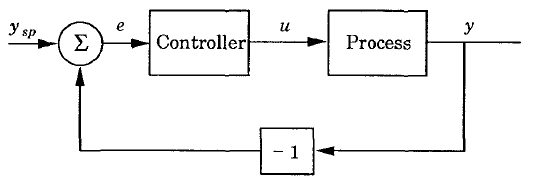
\includegraphics[width=\textwidth]{feedback}
  \caption{Δομικό διάγραμμα μιας διεργασίας με αρνητική ανάδραση}
  \label{fig:feedback}
\end{figure}

\subsection{Αναλογικός Όρος} \label{subsec:proportional_control}

Ο αναλογικός όρος παράγει ένα σήμα εξόδου το οποίο είναι ανάλογο στην τρέχουσα τιμή του σφάλματος. Αυτό επιτυγχάνεται πολλαπλασιάζοντας το σφάλμα $e(t)=y_{sp}-y$ με ένα συντελεστή $K_p$ που ονομάζεται αναλογική σταθερά κέρδους (\emph{proportional gain constant}). Ο αναλογικός όρος συνεπώς δίνεται από τη σχέση:
\begin{equation}
P_{out}=K_p e(t)
\label{eq:p_out}
\end{equation}
Ένα υψηλό αναλογικό κέρδος έχει ως αποτέλεσμα μια μεγάλη αλλαγή στην έξοδο για μια δεδομένη αλλαγή στο σφάλμα. Εάν το αναλογικό κέρδος είναι πολύ υψηλό, το σύστημα μπορεί να γίνει ασταθές (βλ. Το τμήμα σχετικά με τη ρύθμιση βρόγχου). Σε αντίθεση, ένα μικρό κέρδος έχει ως αποτέλεσμα μια μικρή απόκριση εξόδου σε ένα μεγάλο σφάλμα εισόδου και έναν λιγότερο ανταποκρίσιμο ή λιγότερο ευαίσθητο ελεγκτή. Αν το αναλογικό κέρδος είναι πολύ χαμηλό, η ενέργεια ελέγχου μπορεί να είναι πολύ μικρή όταν οφείλεται σε διαταραχές του συστήματος. Στις περισσότερες εφαρμογές ελέγχου, ο αναλογικός όρος είναι αυτός που συνεισφέρει το μεγαλύτερο μέρος στην έξοδο του ελεγκτή.

Επειδή ο αναλογικός όρος επιδρά στην τρέχουσα τιμή του σφάλματος, ένας αναλογικός ελεγκτής πάντα παρουσιάζει ένα σφάλμα μόνιμης κατάστασης (\emph{steady state error}). Εξαίρεση αποτελεί η περίπτωση που η επιθυμητή τιμή είναι η τιμή στην οποία ο αναλογικός όρος ισούται με το μηδέν. Στο Σχήμα \ref{fig:proportional} φαίνεται η επίδραση μόνο του αναλογικού όρου σε μια διεργασία. Για την εξάλειψη του σφάλματος μόνιμης κατάστασης χρησιμοποιούμε τον όρο που αναφέρεται στη συνέχεια.

\begin{figure}[h]
  \centering
  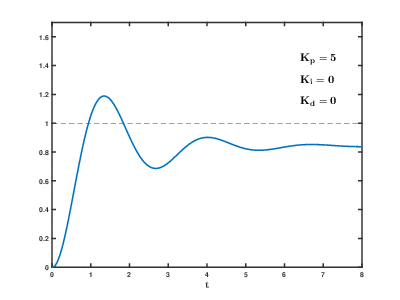
\includegraphics[width=\textwidth]{proportional}
  \caption{Επίδραση του αναλογικού όρου σε μια διεργασία}
  \label{fig:proportional}
\end{figure}

\subsection{Ολοκληρωτικός Όρος}

Η συμβολή του ολοκληρωτικού όρου είναι ανάλογη τόσο με το μέγεθος του σφάλματος όσο και με τη διάρκεια του. Το ολοκλήρωμα ενός ελεγκτή PID είναι το άθροισμα του στιγμιαίου σφάλματος με την πάροδο του χρόνου και δίνει τη συσσωρευμένη μετατόπιση που θα έπρεπε να είχε διορθωθεί προηγουμένως. Το συσσωρευμένο σφάλμα στη συνέχεια πολλαπλασιάζεται με το ολοκληρωτικό κέρδος ($K_i$) και προστίθεται στην έξοδο του ελεγκτή. Ο ολοκληρωτικός όρος δίνεται από τη σχέση:
\begin{equation}
I_{out}=K_i \int_{0}^{t} e(\tau)d\tau
\label{eq:i_out}
\end{equation}
όπου $\tau$ είναι η μεταβλητή ολοκλήρωσης και παίρνει τιμές από το $0$ έως την τρέχουσα χρονική στιγμή $t$. Έτσι, αν η εφαρμοζόμενη δράση δεν είναι αρκετή για να φέρει το σφάλμα στο μηδέν, αυτή η δράση θα αυξηθεί με το πέρασμα του χρόνου. Επίσης ο ολοκληρωτικός όρος επιταχύνει την κίνηση της process variable προς την επιθυμητή τιμή. Ένας καθαρός ολοκληρωτικός ελεγκτής ``I" θα μπορούσε να φέρει το σφάλμα στο μηδέν, ωστόσο θα είχε πολύ αργή αντίδραση στην αρχή (επειδή η δράση θα ήταν μικρή, και θα χρειαζόταν χρόνο για να γίνει σημαντική), βίαιη (η δράση αυξάνεται όσο το σφάλμα είναι θετικό, ακόμη και αν το σφάλμα έχει αρχίσει να πλησιάζει το μηδέν) και αργή να τελειώσει (όταν το σφάλμα αλλάζει πρόσημο, αυτό για κάποιο χρονικό διάστημα μόνο θα μειώνει τη δύναμη της δράσης του ελεγκτή και δε θα το κάνει να αλλάζει και αυτή πρόσημο), προκαλώντας υπέρβαση και ταλαντώσεις. Επιπλέον, θα μπορούσε να προκαλέσει το σύστημα να αποκριθεί ακόμα και αν υπάρχει ήδη μηδενικό σφάλμα καθώς θυμάται ότι το σύστημα είχε σφάλμα και έτσι θα μπορούσε να προκαλέσει μια ενέργεια όταν αυτή δεν είναι απαραίτητη. Το Σχήμα \ref{fig:integral} δείχνει πώς η προσθήκη ενός ολοκληρωτικού όρου εξαλείφει το σφάλμα μόνιμης κατάστασης που δεν κατάφερε να εξαλείψει ο αναλογικός όρος αλλά ταυτόχρονα εισάγει ταλαντώσεις στο σύστημα.

\begin{figure}[h]
  \centering
  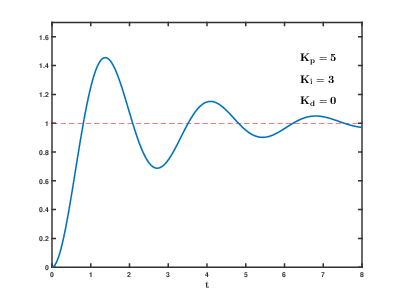
\includegraphics[width=\textwidth]{integral}
  \caption{Εφαρμογή του ολοκληρωτικού όρου στην προηγούμενη απόκριση κρατώντας το αναλογικό κέρδος σταθερό}
  \label{fig:integral}
\end{figure}

\subsection{Παράγωγος Όρος}

Η παράγωγος του σφάλματος της διαδικασίας υπολογίζεται καθορίζοντας την κλίση του σφάλματος με την πάροδο του χρόνου και πολλαπλασιάζοντας αυτόν τον ρυθμό μεταβολής με το κέρδος του παραγώγου $K_d$. Το μέγεθος της συμβολής του παραγώγου όρου στη συνολική δράση ελέγχου ονομάζεται παράγωγο κέρδος (\emph{derivative gain}), $K_d$. Ο παράγωγος όρος δίνεται από τη σχέση:
\begin{equation}
D_{out}=K_d \frac{de(t)}{dt}
\label{eq:dout}
\end{equation}
Ένας παράγωγος όρος δεν λαμβάνει υπόψιν του το σφάλμα (αυτό σημαίνει ότι δεν μπορεί να το φτάσει στο μηδέν: ένας καθαρός ελεγκτής ``D" δεν μπορεί να φέρει το σύστημα στην επιθυμητή τιμή του), αλλά το ρυθμό αλλαγής του σφάλματος, προσπαθώντας να φέρει αυτόν τον ρυθμό στο μηδέν. Στόχος του είναι η τροχιά του σφάλματος να γίνει μια οριζόντια γραμμή, αποσβένοντας την εφαρμοζόμενη δύναμη και μειώνοντας έτσι την υπέρβαση (\emph{overshoot}). Η εφαρμογή υπερβολικής ώθησης όταν το σφάλμα είναι μικρό και συνεχίζει να μειώνεται θα οδηγήσει σε υπέρβαση. Μετά την υπέρβαση, αν ο ελεγκτής εφαρμόσει μια μεγάλη διόρθωση στην αντίθετη κατεύθυνση και επανειλημμένα υπερβεί την επιθυμητή θέση, η έξοδος θα ταλαντώνεται γύρω από την επιθυμητή τιμή είτε σε ένα σταθερό, αναπτυσσόμενο ή σε αποσβεννούμενο ημιτονοειδές. Εάν το πλάτος των ταλαντώσεων αυξάνεται με το χρόνο, το σύστημα είναι ασταθές. Εάν μειώνεται, το σύστημα είναι σταθερό. Εάν οι ταλαντώσεις διατηρούν σταθερό πλάτος, το σύστημα είναι οριακά σταθερό. Ο παράγωγος όρος προβλέπει τη συμπεριφορά του συστήματος και επομένως βελτιώνει τον χρόνο που απαιτείται για να ηρεμήσει το σύστημα (\emph{settling time}) καθώς και τη σταθερότητα του συστήματος \cite{michigan}, \cite{wescott}. Ένα ιδανικός παράγωγος ελεγκτής δεν είναι αιτιατός, και έτσι οι εφαρμογές των PID ελεγκτών περιλαμβάνουν ένα πρόσθετο φίλτρο χαμηλής διέλευσης (\emph{low-pass filter}) για τον παράγωγο όρο για να περιορίσουν το κέρδος και το θόρυβο υψηλής συχνότητας. Ο παράγωγος όρος χρησιμοποιείται πολύ πιο σπάνια στην πράξη από τους άλλους δύο όρους (P και I), λόγω της μεταβλητής επίδρασής του στη σταθερότητα του συστήματος σε πραγματικές εφαρμογές. Το Σχήμα \ref{fig:derivative} δείχνει πώς βελτιώθηκε η συνολική απόκριση του συστήματος και εξαλείφθηκαν οι ταλαντώσεις που είχε εισάγει ο ολοκληρωτικός όρος με την προσθήκη του όρου παραγώγου.

\begin{figure}[h]
  \centering
  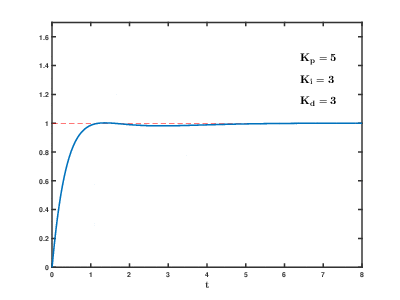
\includegraphics[width=\textwidth]{derivative}
  \caption{Εφαρμογή του όρου παραγώγου στην προηγούμενη απόκριση κρατώντας τα άλλα κέρδη σταθερά}
  \label{fig:derivative}
\end{figure}

\subsection{Εξίσωση του PID ελεγκτή}

Οι τρεις όροι που αναλύθηκαν παραπάνω είναι αυτοί που δίνουν στον ελεγκτή το όνομά του. Το άθροισμα των τριών αυτών όρων αποτελεί τη μεταβλητή που μεταχειρίζεται ο ελεγκτής (\emph{manipulated variable}) και ισούται με την έξοδό του. Ορίζοντας ως $u(t)$ την έξοδο του ελεγκτή και αθροίζοντας τις εξισώσεις \ref{eq:p_out}, \ref{eq:i_out} και \ref{eq:dout} η τελική μορφή του είναι:
\begin{equation}
u(t)=MV(t)=K_p e(t) + K_i \int_{0}^{t} e(\tau)d\tau + K_d \frac{de(t)}{dt}
\label{eq:parallel_pid}
\end{equation}
Αυτή η μορφή του PID είναι γνωστή ως παράλληλη (\emph{parallel}). Η μορφή του PID που χρησιμοποιείται περισσότερο στη βιομηχανία και η οποία χρησιμοποιήθηκε και σε αυτή την εργασία είναι η τυποποιημένη μορφή (\emph{standard form}). Σε αυτή τη μορφή το κέρδος του αναλογικού όρου $K_p$ εφαρμόζεται και στους άλλους δύο όρους και έτσι η εξίσωση που προκύπτει είναι η:
\begin{equation}
u(t)=MV(t)=K_p \left( e(t) + \frac{1}{T_i}\int_{0}^{t} e(\tau)d\tau + T_d\frac{de(t)}{dt} \right)
\label{eq:standard_pid}
\end{equation}
όπου $\boldsymbol{T_i}$ είναι ο χρόνος ολοκλήρωσης και $\boldsymbol{T_d}$ είναι ο χρόνος παραγώγισης. Σε αυτή τη μορφή, οι παράμετροι έχουν σαφή φυσική σημασία. Συγκεκριμένα, η εσωτερική άθροιση παράγει μια νέα μοναδική τιμή σφάλματος η οποία αντισταθμίζεται για μελλοντικά και παρελθόντα σφάλματα. Η προσθήκη των αναλογικών και παραγώγων συνιστωσών προβλέπει την τιμή σφάλματος σε $T_d$ δευτερόλεπτα (ή δείγματα) στο μέλλον, υποθέτοντας ότι ο έλεγχος βρόχου παραμένει αμετάβλητος. Το ολοκληρωτικό στοιχείο προσαρμόζει την τιμή σφάλματος για να αντισταθμίσει το άθροισμα όλων των παρελθόντων σφαλμάτων, με σκοπό την πλήρη εξάλειψή τους $T_i$ δευτερόλεπτα (ή δείγματα). Η προκύπτουσα αντισταθμισμένη τιμή μοναδικού σφάλματος κλιμακώνεται από το μοναδικό κέρδος $K_p$.

Οι συντελεστές της εξίσωσης (\ref{eq:parallel_pid}) με αυτούς της εξίσωσης (\ref{eq:standard_pid}) συνδέονται με τις σχέσεις: $\boldsymbol{K_i=\frac{K_p}{T_i}}$ και $\boldsymbol{K_d=K_p T_d}$. Η παράλληλη μορφή, όπου οι παράμετροι αντιμετωπίζονται ως απλά κέρδη, είναι η πιο γενική και ευέλικτη μορφή. Ωστόσο, είναι επίσης η μορφή όπου οι παράμετροι αυτοί έχουν τη λιγότερη φυσική ερμηνεία και γενικά προορίζονται για θεωρητική ανάλυση του PID ελεγκτή. Η τυποποιημένη μορφή, παρά το γεγονός ότι είναι λίγο πιο περίπλοκη μαθηματικά, είναι πιο συνηθισμένη στη βιομηχανία.

\paragraph{\fbox{Σύνοψη}}
Ο PID ελεγτκής έχει τρεις όρους. Ο αναλογικός όρος (\emph{``P"}) αφορά τον αναλογικό έλεγχο και επιδρά στο τρέχον σφάλμα. Ο ολοκληρωτικός όρος (\emph{``I"}) παρέχει μια δράση ελέγχου που είναι ανάλογη στο χρονικό ολοκλήρωμα του σφάλματος. Αυτό εξασφαλίζει ότι το σφάλμα μόνιμης κατάστασης γίνεται μηδενικό. Ο παράγωγος όρος (\emph{``D"}) είναι ανάλογος της χρονικής παραγώγου του σφάλματος. Αυτός ο όρος προβλέπει το μελλοντικό σφάλμα. Εκτός από αυτές τις δύο μορφές του PID υπάρχουν και άλλες, η καθεμία με διαφορετικές ιδιότητες αλλά οι δύο που αναφέρθηκαν είναι οι πιο γνωστές. Κάποιος που θέλει να μελετήσει και τις άλλες μπορεί να απευθυνθεί στην πηγή \cite{astrom}.

\subsection{Τροποποιήσεις του PID αλγορίθμου}

\subsubsection{Integral Windup}
Όταν σχεδιάζεται ένας πρακτικός PID ελεγκτής που θα ελέγχει πραγματικούς ενεργοποιητές όπως βαλβίδες, διακόπτες κτλ, θα πρέπει να λαμβάνονται υπόψιν και οι περιορισμοί του εξοπλισμού αυτού. Για παράδειγμα ένας κινητήρας έχει περιορισμένη ταχύτητα, μια βαλβίδα έχει όρια στο πόσο ανοιχτή ή πόσο κλειστή μπορεί να είναι και ούτω καθεξής. Συνεπώς, αν ένα σύστημα δεν μπορεί να φτάσει την επιθυμητή τιμή χωρίς να ξεπεράσει αυτά τα όρια τότε θα υπάρχει πάντα ένα σφάλμα μόνιμης κατάστασης, ακόμα και αν έχει προστεθεί ο ολοκληρωτικός όρος στον PID ελεγκτή. Αυτό έχει σαν αποτέλεσμα ο ολοκληρωτικός όρος να συνεχίζει να συσσωρεύει σφάλμα και έτσι αυτός μπορεί να γίνει πολύ μεγάλος και να οδηγήσει το σύστημα σε ανεπιθύμητη συμπεριφορά. Αυτό αναφέρεται στη διεθνή βιβλιογραφία ως \textbf{\emph{integral windup}}. Αυτό το πρόβλημα μπορεί να αντιμετωπιστεί με κάποια από τις ακόλουθες τροποποιήσεις στο βασικό αλγόριθμο:
\begin{itemize}
\item Απενεργοποίηση της ολοκλήρωσης έως ότου η μεταβλητή της διεργασίας εισέλθει στην ελεγχόμενη περιοχή
\item Αποτροπή της συσσώρευσης του ολοκληρωτικού όρου πάνω ή κάτω από τα προκαθορισμένα όρια
\item Υπολογισμός εκ των υστέρων του ολοκληρωτικού όρου για τον περιορισμό της εξόδου του ελεγκτή εντός εφικτών ορίων
\end{itemize}

\subsubsection{Bumpless λειτουργία}
Διάφορες αλλαγές μπορεί να επέλθουν σε έναν PID που είναι ενεργός. Μπορεί να αλλάξουν οι παράμετροί του ή να αλλάξει η λειτουργία του από χειροκίνητη σε αυτόματη. Οι ελεγκτές PID υλοποιούνται συχνά με ένα χαρακτηριστικό ``εξομάλυνσης" έτσι ώστε η έξοδός τους να μεταβάλλεται με ομαλό τρόπο κατά τη διάρκεια αυτών των αλλαγών \cite{douglas}.

\subsubsection{Περισσότερες τροποποιήσεις}
Φυσικά μετά από τόσα χρόνια εφαρμογής του PID αλγορίθμου στη βιομηχανία, πολλές εναλλακτικές μορφές του έχουν προταθεί, πέρα από αυτές τις δύο προαναφερθέντες. Η καθεμία από αυτές τις τροποποιήσεις βελτιώνει πολλά από τα προβλήματα του βασικού αλγορίθμου. Κάποιος που θέλει να ενημερωθεί για όλες τις τροποποιήσεις του αλγορίθμου αναλυτικά, καλείται να ανατρέξει στην πηγή \cite{astrom}.

%\section{Ρύθμιση του PID ελεγκτή}
%
%\lettrine[findent=2pt]{\fbox{\textbf{Η}}}{} ρύθμιση του PID ελεγκτή έχει να κάνει με την απόδοση τιμών στο συντελεστή κάθε όρου, έτσι ώστε καθένας από αυτούς να επηρεάσει θετικά την απόκριση του συστήματος, ενώ ταυτόχρονα να μετριαστούν όσο γίνεται περισσότερο τα αρνητικά του κάθε όρου. Ο τύπος της διεργασίας επηρεάζει το τι είναι επιθυμητό από τον έλεγχό της. Για παράδειγμα, κάποιες διεργασίες μπορεί να μην ανέχονται υπέρβαση (\emph{overshoot}) της απόκρισής τους και αυτό να θέτει και περιορισμούς στο χρόνο ανύψωσης (\emph{rise time}). Αντιθέτως, άλλες διεργασίες μπορεί να παρουσιάζουν ανοχή σε ένα ποσοστό υπέρβασης και έτσι να επιτρέπουν να αυξηθεί ο χρόνος ανύψωσης. 

%Φυσικά ένας ελεγκτής με την ευρεία και διαδεδομένη χρήση όπως αυτή του PID θα είχε πολλές ακόμα τροποποιήσεις στον αλγόριθμό του. Πράγματι υπάρχουν πολλές υλοποιήσεις του PID αλγορίθμου που η καθεμία προσφέρει λύση σε διαφορετικό πρόβλημα του βασικού PID αλγορίθμου. Τα δύο παραπάνω προβλήματα αναφέρθηκαν συγκεκριμένα επειδή η αντιμετώπισή τους είχε ρόλο στην επιλογή του PID αλγορίθμου που χρησιμοποιήθηκε σε αυτή την εργασία. Κάποιος που θέλει να ενημερωθεί για όλες τις τροποποιήσεις του αλγορίθμου αναλυτικά, καλείται να ανατρέξει στην πηγή \cite{astrom}.

%\lettrine[findent=2pt]{\fbox{\textbf{Κ}}}{ατά} την αποτύπωση οποιουδήποτε αναλογικού σήματος $S(t)$ σε ψηφιακή μορφή $S_i$, πραγματοποιείται μια διαδικασία που ονομάζεται \emph{δειγματοληψία (sampling)} κατά την οποία ένα συνεχές σήμα γίνεται διακριτό και στη συνέχεια εφαρμόζουμε \emph{κβαντισμό} στις τιμές του, για να περάσουμε σε ψηφιακή αναπαράσταση. Όπως φαίνεται και στο σχήμα \ref{fig:sampling}, σε διακριτές χρονικές στιγμές λαμβάνουμε την τιμή του αναλογικού σήματος (μέσω ενός μετατροπέα Αναλογικού σε Ψηφιακό (ADC)) κι έτσι δημιουργούμε μια σειρά από τιμές (\emph{δείγματα}) τα οποία έχουν συγκεκριμένη και σταθερή χρονική απόσταση $T_s$. Η χρονική απόσταση έχει νόημα μόνο ως προς το αναλογικό σήμα, ενώ στην ψηφιακή μορφή των δειγμάτων αναφερόμαστε σε αυτά με ένα δείκτη $n$ και μεταξύ αναλογικού και ψηφιακού σήματος ισχύει ότι $S_i=S(nT_s)$.
%\begin{figure}[h]
%  \centering
%  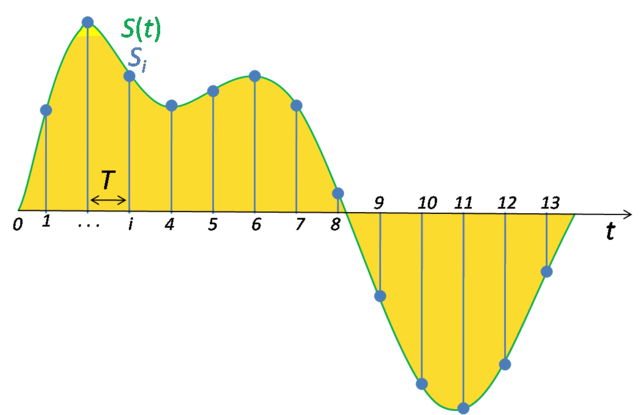
\includegraphics[width=0.6\textwidth]{Signal_Sampling}
%  \caption{Δειγματοληψία ενός αναλογικού σήματος}
%  \label{fig:sampling}
%\end{figure}
%Κατά τη δειγματοληψία ``χάνουμε'' αρκετή από την πληροφορία που περιέχει το αναλογικό σήμα, καθώς οι τιμές που βρίσκονται μεταξύ των διαστημάτων $T_s$ όπου λαμβάνουμε δείγματα δε λαμβάνονται υπόψη. Ακόμη, λόγω της πεπερασμένης ακρίβειας των ψηφιακών συστημάτων για αναπαράσταση αριθμών, η τιμή που έχει το σήμα στρογγυλοποιείται στην πλησιέστερη (είτε μεγαλύτερη είτε μικρότερη) τιμή που μπορεί να αναπαραστήσει το σύστημά μας.
%
%Όπως γίνεται αντιληπτό, σε πολλές των περιπτώσεων η δειγματοληψία μπορεί να έχει καταστροφικές συνέπειες για το αναλογικό σήμα. Ωστόσο, υπό προϋποθέσεις, μπορεί να είναι αντιστρεπτή διαδικασία -- μπορούμε δηλαδή από τα δείγματα που έχουμε λάβει να επιστρέψουμε στην αναλογική μορφή του σήματος. Οι προϋποθέσεις αυτές ορίζονται από το θεώρημα \emph{Shannon-Nyquist} (\ref{thrm:shannon-nyquist}), ως:
%\\
%\begin{theorem}[Shannon-Nyquist]
%	\label{thrm:shannon-nyquist}
%	Ένα σήμα με μέγιστη συχνότητα $f_{max}$ μπορεί να ανακτηθεί από τα δείγματά του, αν αυτά ληφθούν με συχνότητα $f_s>2f_{max}$, ή αλλιώς με περίοδο $T_s<\frac{1}{2f_{max}}$. \cite{proakis_sampling}
%\end{theorem}
